\documentclass[10pt,a4paper,oneside]{article}
\usepackage[latin1]{inputenc}   % St�tte for direkte input av norske tegn
\usepackage{graphicx}
\begin{document}

\begin{titlepage}

\emph{Rendering based on hybrid methods}

by Torbj�rn Haugen and P�l Solberg Trefall
\today

\begin{figure}[htbp]
	\centering
		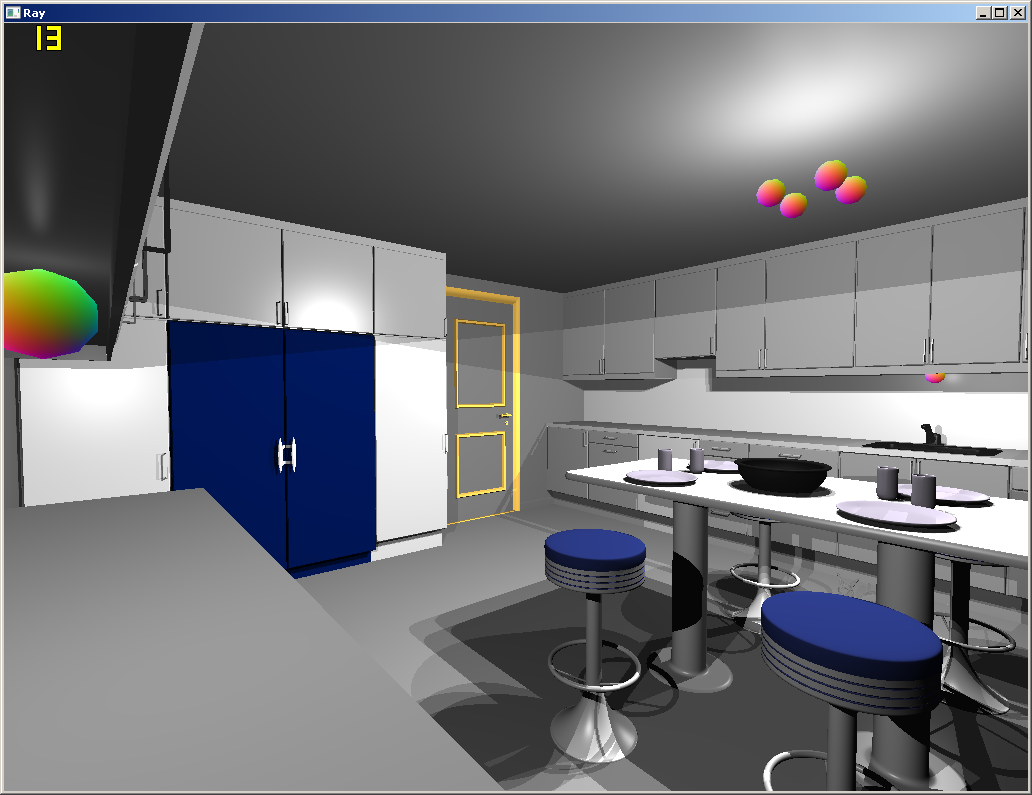
\includegraphics[width=0.90\textwidth]{0/all_lights.png}
	\caption{BART Kitchen}
	\label{fig:all_lights}
\end{figure}

\end{titlepage}

\begin{abstract}
We are going to study various rendering techniques, and compare them to a renderer that combines deferred shading and raytracing.
\end{abstract}

\tableofcontents

%
% special latex characters: # $ % ^ & _ { } ~ \
% can be added in your documents using a prefix backslash

\section{latex sandbox}

\#

\$


\part{Previous work}

There are few commercial rendering engines that combine rasterization and raytracing. Virtually all computer games use rasterization. The demand for graphical fidelidy has driven the development of programmable GPUs. For some time now, it has been possible to implement direct/Whitted-style and pathtracing on a GPU.

Exampels of real time direct raytracing engines. Manta, Razor, Arauna.
Examples of real time path tracing engines. SmallPT, Brigade.

Examples of hybrid engines; Pixar's REYES

\paragraph{Hybrid shadows} renders world space positions to a texture. Texture is loaded into optix, from there a ray is traced from each world space position against all lights. Attenuates given world space position and saves attenuation value in a shadowmap.

\paragraph{ISG Shadows} Image Space Gathering \cite{nvidiarobison09}
\paragraph{ISG Reflection}


\section {Global Illumination (GI) techniques}
	\subsection{Pure raytracing} 
		One pass. But produces ugly hard shadows unless we shoot more that one shadowray.
	\subsection{Photon mapping} A two pass algorithm. Combines ray tracing and particle tracing.
		\paragraph{1.st pass} photons are cast from the light source and checkt for intersection against the scene.    Every intersecting photon is stored in a photon map. After intersecting the scene a photon may be reflected, refracted or absorbed depending on the material properties of the surface. The selection is done by the Monte Carlo method called 'russian roulette'. If the photon is not absorbed, then a new traveling direction is calculated for it according to the selected behavior.
			
		\paragraph{2.nd pass} View rays are cast from the camera and checked for intersection against the scene similar to raytracing. Once the nearest intersection point is found, a pre-defined number of nearest photons are sampled, and interpolated to calculate irradiance at that point.

	\subsection {Radiosity}
		Diffuse inter-reflections of light in a scene. Divides scene geometry into small
		patches. For every pair of patches, one defines a camera model for how they can
		see each other. Ex: paraboloid, cuboid-mapping. These form factors are then used
		in an iterative process that progressively transfers radiation between the
		patches.

		Can generate realistic diffuse lighting and is viewpoint independant. As long as
		geometry and lightsources remain unchanged, the simulation can be effectively
		sotred and sampled to obtain the scene lighting for any view.

		Con: Limited diffuse lighting effects. Can't do absorb, refract?

	\subsection {Instant Radiosity}
		A technique developed by Alexander Keller to approximate the simulation of light
		transfers between purely diffuse surfaces. The algorithm goes as follows, first
		one casts a large quantity of rays from each light in random directions which
		are then checked for intersection against the scene. Then, at the intersection
		point create a so called 'virtual point light' (VPL). These VPLs represent the
		light bouncing off surfaces. Accuracy may be improved by recursively casting new
		light rays from each VPL, but one step usually creates a reliable approximation.
		Once the VPLs have been created, they are rendered as normal point lights.
		Modern GPUs are very good at this.

	\subsection {Path Tracing}
		Path tracing combines ray tracing and Monte Carlo methods to approximate the
		integral of incoming light at each point. It is one of the most physically
		accurate methods, but also one of the most demanding ones in terms of
		computations. Path tracing is naturally capable of generating effects like depth
		of field, caustics and soft shadows. The idea is to cast many rays at each
		intersection. The number of rays is decided by the properties of the intersected
		surface, for example its BRDF. If we as an example take a diffuse surface, then
		rays are distributed on the hemisphere above the intersection point. But, if the
		surface is glossy, then the generated rays are distributed around the reflection
		vector. There are many methods that improve the performance of this brute force
		method, such as stratified sampling, importance sampling and a modification
		called 'Bidirectional Path Tracing' that is useful to increase the chance of a
		ray intersecting a surface in scenes with small or occluded light sources.

\section {Real-time Global Illumination}
	Recent advancements were made by taking classical algorithms and implementing
	them on GPUs. These effects have been adapted to rasterization, examples are:
	ambient occlusion, soft shadows, depth-of-field, atmospheric scattering and water reflections and refractions.

	\subsection {Screen Space Ambient Occlusion}
		Screen Space Ambient Occlusion (SSAO) is a technique that was recently pioneered by Crytek. It approximates ambient occlusion in real-time on the gpu. The technique is decoupled from the scene complexity and requires a smaller amount of rays than the original ambient occlusion technique. It relies entirely on the depth buffer, this means geometry outside whats visible can not cause occlusion.

	\subsection {Screen Space Global Illumination}
        Screen Space Global Illumination (SSGI) is an extension of SSAO that generates a rough approximation of global illumination on a small scale. SSGI works by sampling colors from the rendered image of the scene to simulate secondary light bounces, it there for suffers from the same limitations as SSAO, so it can only show light interactions between objects that are very close to each other. Despite these limitation it is useful when combined with a coarse global illumination technique like instant radiosity. This way, SSGI can provide high-frequency global illumination and instant radiosity provides coarse, low-frequency global illumination.

	\subsection {Image Space Photon Mapping}
		The photon mapping algorithm has been adapted for real-time use in an algorithm called image space photon mapping (ISPM), that generates the information about the first bounce of photons on the GPU using Reflective Shadow Maps (RSM). \cite{dachsbacher2005} 
		From this initial distribution of photons, a reduced set is selected and recursively raytraced on the CPU similarily to original photon mapping. The consecutive bouncing of each photon is stored and sent back to the GPU for rendering. On the GPU, the photons are used to estimate lighting using a scattering approach, the opposite of the gathering approach used by classical photon mapping. The scattering is performed by rendering ellipsoid-shaped volumes in screen space that represent the influence of each photon on the pixels around it. For each pixel affected by the photon volume, the scene properties are sampled and the lighting contribution of that photon is computed for that pixel. ISPM is capable of mathematically identical results to traditional photon mapping as long as it is rendered at full screen resolution.

		\begin{figure}
			\centering
				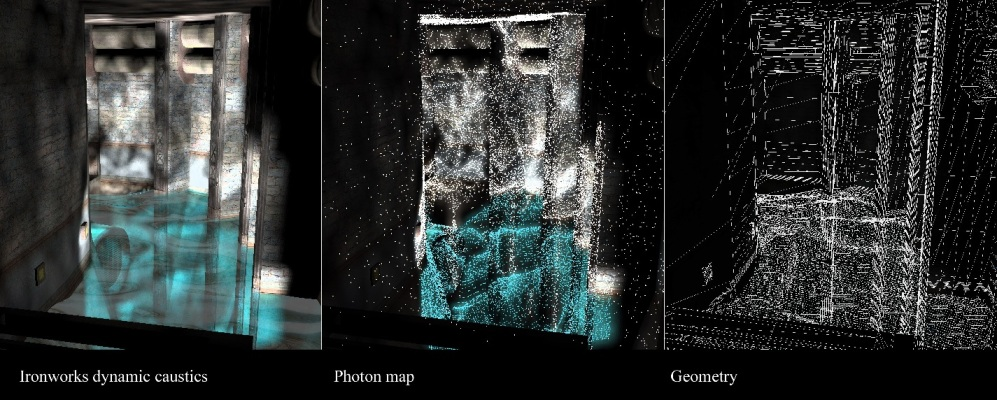
\includegraphics[width=1.00\textwidth]{previous_work/ispm.jpg}
			\caption{McGuire and Luebke's ISPM extension}
			\label{fig:ispm}
		\end{figure}

	\subsection {Global Illumination with Light Propagation Volumes}

	Global Illumination with Light Propagation Volumes (LPV) is a technique for approximation instant radiosity on the GPU. \cite{kaplanyan2009} This technique avoids the instant radiosity requirements for processing a large amount of lights by using a representation of the scene lighting that decouples scene illumination from light quantity. The first step is to generate an initial distribution of VPLs, this is done by rendering a Reflective Shadow Map (RSM) \cite{dachsbacher2005} from the lights point of view. The radiance of each VPL is injected as spherical harmonics into a 3D texture as spherical harmonics that represents the initial distribution of radiance on the scene. Then the initial radiances are propagated iteratively through the radiance volume to simulate light propagation. The volume is then sampled once per-pixel to obtain the irradiance at that location.

\subsection {Real-Time Ray Tracing}
	Inigo Wald. SIMD. packet tracing. openRT. 
	\paragraph{Arauna} uses kd-tree for static. bih for dynamic.

\subsection {Real-Time Path Tracing}
	One of the most complex global illumination algorithms. 
	\paragraph {Nvidia Optix} demonstration
	\paragraph {Brigade} 
	\paragraph {V-ray}

\subsection {Combining Rasterization and Ray Tracing}

Rasterization and Ray Tracing are very different, but can be combined to exploit each ones strengths. Rasterization is good at direct lighting, while raytracing is flexible for many effects.

\subsubsection {RenderMan}

By Pixar.

% part c
% chapter % funker ikke for article virker det som section subsection
% subsubsection 
% paragraph 
% subparagraph

\part{OpenGL 3.0+}

We have used GL 3+ functions only. Limiting the program to GL3.0+ core also simplifies interop with Optix.

Pixel Buffer Objects PBO
\section{OptiX}

\subsection{Introduction}
OptiX is a closed source raytracing engine designed by Nvidia, and currently only works on their own GPUs. The library is free to use both for hobbyists and for commerce. One can speculate that it will be opened up further once equivalent vendor agnostic libraries become available.

Optix can be seen as a framework for launching rays. It doesn't know anything about lights, shadows, ambient occlusion or any other rendering detail for that matter. What it does know is; rays, how to build and traverse acceleration structures, geometry representation and how to traverse the scene.What makes OptiX interesting is programmability; a variety of ray tracing-based algorithms in graphics and non-graphics domains can be implemented \cite{Parker10OptiX} by creating custom programs.

\subsection{Programs}
\paragraph{There are eight} different types of user provided programs in OptiX. These programs are implemented using the CUDA C-language. They all operate on a single ray at a time, except for the bounds program, which is used to determine bounds for acceleration structure construction. For triangle geometry, Optix can access individual vertices of a mesh for constructing a k-dimensional-tree (kdtree) or split bounding volume hierarchy  (sbvh).

\begin{enumerate}
	\item {
	\textbf{Ray generation}
      programs (``raygen'' from here on) are launched by the client program using rtContextLaunch(rayProgramIndex, with, height). This invokes many raygen programs in parallel. The raygen is the main entry point into the raytracing pipeline. Input and output buffers are declared inside. You can use a single raygen program as a general compute shader, but the intended use is to implement a camera model by initializing ray origin and direction. After a ray has been initialized, \begin{verbatim}rtTrace startNode,ray,payload \end{verbatim} can be called, and will trace all of start nodes children. 
	}

	\item{\textbf{Exeption} programs are invoked when the system encounters problems like out of stack space, or buffer access index is                   out of range. Also supports user-defined exceptions that can be 	thrown from any program. Can react by printing                         diagnostic messages or   writing specific color values to an output buffer.}

	\item{\textbf{Closest hit} programs are invoked once traversal has found the closest intersection of a ray with scene geometry.}

	\item{\textbf{Any hit}
		allow shading to be kept separate from geometry.
		May call rtTerminateRay and stop all traversal. Early ray termination for shadowrays and AO.
		Also useful for binary transparency by texture look up.
		Default any hit program is a no-op, often the most desired operation.
		}

	\item{\textbf{Miss} intersect any geometry. }

	\item {\textbf{Intersection}
	programs are needed to describe geometry. The program must at least report if and where the ray touches the object, 
	additional computations may involve normals, texture coordinates and other attributes based on hit position.
	Intersection programs allow you to trace perfect spheres, cylinders, cubes,  CSG-surfaces, parametric surfaces like
	Bezier and NURBS, fractals and of course triangle meshes. Parker \cite{Parker10OptiX} notes \begin{quote} programmable intersection op-
	eration facilitates direct access to the native format, which can help
	avoid copies when interoperating with rasterization-based systems.\end{quote} In our program we store vertex attributes continuously (first all positions, then all normals, etc.) as opposed to storing them interleaved (one position, one normal and so on). Unfortunately, the built in acceleration sbvh and kdtree builders expect triangle geometry to be interleaved, so we settled for the generic bvh builder.
	}
	
	\item{\textbf{Selector}
		visit programs gives on control over graph traversal.
		The program can do traversals based on data stored in a visitor programs payload and make a traversal decision based 	on that data.
	}

 \item{\textbf{Bounding box}
		programs obviously compute the bounds associated with each primitive to enable acceleration structures over any geometry. The bounding box program takes a primtive index and computes its bounds. From the client api, a node is associated a given bounds program.
	}
 				
\end{enumerate}

The closest hit, any hit and miss programs determine shading. The raygen, selector and intersection programs determine scene traversal.
			 
\subsection{Client-side API}

To begin raytracing a scene ``rtContextLaunch( raygenIdx, width, height )'' is called with a given Rey Generation Program index as a parameter. From the ray generation program ``rtTrace( rootNode, ray, payload )'' is given the root scene node for traversal. During traversal, if a node a nodes associated selector and acceleration program is run.
If the acceleration traverser determines that a primitive node is hit, it invokes the primitives intersection program.
If the Intersection program calls ``rtReportIntersection'', the primitives associated ``material'' Any Hit Program is called.
If the ray doesn't hit anything, a miss program is called. The missprogram is always required.

\subsection{CUDA program API}

\paragraph{A simple raygen program:}

\begin{verbatim}
// notice use of templates for type and dimension
rtBuffer<unsigned char, 2> outputBuffer; 

RT_PROGRAM void pinhole_camera() {
  Ray ray = PinholeCamera::makeRay( launchIndex );
  UserPayload payload;
  rtTrace( topObject, ray, payload );
  outputBuffer[launchIndex] = payload.result;
}
\end{verbatim}


\section{OptiX and GL interopability}


Combining our deferred raster pipeline with OptiX can either be done from scratch, learning what every OptiX API-call does, or, copy one of the GL/Optix interop examples and modify it until it works. 

\subsection{Shared State}

The following state must be synchronized between GL and OptiX

\begin{enumerate}
	\item Geometry and its transform (model matrix)
	\item Textures (if we find that they can demonstrate any advantages)
	\item Camera (view matrix \& projection matrix)
\end{enumerate}

For geometry, ``optix::Context'' provides functions createBufferFromGLBO and similar createTextureSamplerFromGLImage for textures.

The standard pinhole\_camera.cu implementation is used, then the view vectors (u,v,w) must be extracted from our camera class or the modelview matrix.

\paragraph{Description of the rendering pipeline}

GL and OptiX scenes are independently rendered. We end up with two sets of g-buffers, shading and composition is done in a shader.


\section{Our hybrid renderer}


\subsection{Deferred pipeline}

\subsection{CameraModel}
The raytracer uses pinhole camera model. The eye is a point, rays are cast from this point, through the viewplane and into the scene. Eyepoint-viewplane distance determines focal length. A rasterizer on the other hand requires a projection matrix.

\subsection{Various hybrid configurations}

\subsection{Geometry}

Traditional triangle meshes with vertex attributes (normals, texture coordinates etc)



\section{Further work}

The work presented in this thesis can be improved. 
\begin{itemize}
	\item We identified that graphics hardware drivers are still not handling interoperation between Cuda and OpenGL fast enough. Using OpenGL 4.3, a raytracer could be implemented in the Compute Shader stage, which should cancel the interoperation overhead.
	\item The deferred renderer could be rewritten to take advantage of tile-based parallellization in it's lighting pass. Using OpenGL 4.3, this could also be handled in a Compute Shader now, and probably also integrate well with a Compute Shader based raytracer.
	\item Improve the BART loader to support animations. That would allow us to compare performance with other BART renderers.
	\item Extend the raytracer with intersect programs for geometry that is better suited for raytracing than rasterization, like NURBS, Meta Shapes and Distance Fields.
\end{itemize}


\begin{thebibliography}{9}

%\bibitem{cite_mnemonic}
% Author
% Paper title
% publisher
% edition
% year of publication

\bibitem{nvidiarobison09}
	Robison, Austing and Shirley, Peter,
	Image space gathering,
	HPG '09: Proceedings of the Conference on High Performance Graphics 2009

\bibitem{joao10}
  Jo�o Cabeleira,
	Combining Rasterization and Ray Tracing Techniques to Approximate Global Illumination in Real-Time
  Instituto Superior T�cnico,
  www.voltaico.net
  2010
  
\bibitem{nv2012}
  Nvidia Corporation,
  OptiX Ray Tracing Engine
  Programming Guide version 2.5
  27. January 2012

\bibitem{Parker10OptiX}
  Parker et al.,
  OptiX: A General Purpose Ray Tracing Engine
  ACM 2010
  
\bibitem{Mania2008}
	K. Mania and E. Reinhard
	Improving Interaction Performance for Ray Tracing
	Eurographics Short Paper
	2008

\end{thebibliography}

\end{document}
